% Cuestión II. Toda cifra medida sale de generado/ (\dato o tablas \input); no escribir cifras a mano.

\subsection{Metodología}

El portador es \texttt{Ejemplo/lado.bmp}, un BMP de \dato{portador-ancho}\,$\times$\,\dato{portador-alto} píxeles
y 24 bits por píxel, con \dato{portador-bytes} bytes de datos de imagen y sin relleno al final de cada fila.
Para que la comparación no dependa de un único mensaje se ocultaron tres cargas con cada método:
la imagen PNG que la cátedra escondió en sus propios ejemplos (\dato{png-bytes} bytes, un archivo ya comprimido),
el mensaje de prueba del propio paper~\cite{majeed2015} (\dato{paper-bytes} bytes de texto en inglés, sin
retorno de carro final) y \dato{azar-bytes} bytes pseudoaleatorios, generados de forma determinista con SHA-256,
que hacen de reemplazo de un mensaje cifrado (un buen cifrado produce bytes indistinguibles del azar).
La carga principal es el PNG, y con él se escribieron los comandos:

\begin{lstlisting}
./stegobmp -embed -in catedra.png -p Ejemplo/lado.bmp -out png-LSB1.bmp -steg LSB1
./stegobmp -embed -in catedra.png -p Ejemplo/lado.bmp -out png-LSB4.bmp -steg LSB4
./stegobmp -embed -in catedra.png -p Ejemplo/lado.bmp -out png-LSBI.bmp -steg LSBI
\end{lstlisting}

Cada resultado se extrajo de nuevo con \texttt{-extract} y se comparó byte a byte con la carga original, y los
tres archivos con el PNG se compararon con los ejemplos de la cátedra (\texttt{ladoLSB1.bmp}, \texttt{ladoLSB4.bmp} y
\texttt{ladoLSBI.bmp}): son idénticos byte a byte, de modo que las cifras que siguen describen también la
implementación de referencia. La capacidad máxima de cada método se leyó del mensaje de error que imprime
\texttt{stegobmp} al intentar ocultar un archivo demasiado grande. La distorsión se midió con \texttt{tools/bmpdiff.py}
(bytes y bits modificados, cambios por canal, error cuadrático medio MSE y relación señal-ruido PSNR sobre los bytes
de color) y las huellas estadísticas con \texttt{tools/lsbstats.py} (proporción de bytes con el bit menos significativo
en uno y estadístico $\chi^2$ de pares de valores, por canal, definido como en Westfeld y Pfitzmann~\cite{westfeld2000}).
Todo se regenera con \texttt{make report}, sin intervención manual.

\subsection{Resultados}

El cuadro~\ref{tab:q2-png} resume el caso del PNG. El cuadro~\ref{tab:q2-cargas} repite las mediciones esenciales para las
tres cargas y el cuadro~\ref{tab:q2-estadisticas} muestra las huellas estadísticas por canal del portador original y de
los tres archivos con el PNG.

\begin{table}[htbp]
\centering
\small
\begin{tabular}{lrrr}
\toprule
Métrica & LSB1 & LSB4 & LSBI \\
\midrule
Capacidad máxima (bytes) & 115\,200 & 460\,800 & 76\,799 \\
Bytes ocultados & 44\,895 & 44\,895 & 44\,895 \\
Uso de la capacidad (\%) & 38{,}97 & 9{,}74 & 58{,}46 \\
Bytes del portador usados & 359\,160 & 89\,790 & 359\,164 \\
Bytes modificados & 190\,182 & 85\,370 & 170\,852 \\
Bits modificados & 190\,182 & 205\,965 & 170\,852 \\
Tasa de cambio por byte usado (\%) & 52{,}95 & 95{,}08 & 47{,}57 \\
Bytes modificados sobre el total (\%) & 20{,}64 & 9{,}26 & 18{,}54 \\
Cambio máximo por byte & 1 & 15 & 1 \\
Bytes rojos modificados & 63\,341 & 28\,443 & 0 \\
Último offset modificado & 359\,213 & 89\,843 & 538\,794 \\
MSE & 0{,}2064 & 8{,}7631 & 0{,}1854 \\
PSNR (dB) & 54{,}98 & 38{,}70 & 55{,}45 \\
Idéntico al archivo de la cátedra & sí & sí & sí \\
Extracción correcta & sí & sí & sí \\
\bottomrule
\end{tabular}

\caption{Resultados medidos al ocultar la misma imagen PNG en lado.bmp con cada método}
\label{tab:q2-png}
\end{table}

\begin{table}[htbp]
\centering
\small
\setlength{\tabcolsep}{4pt}
\begin{tabular}{llrrrrr}
\toprule
Carga & Método & Ocultos & Uso (\%) & Modificados & Tasa (\%) & PSNR (dB) \\
\midrule
Imagen PNG & LSB1 & 44\,895 & 38{,}97 & 190\,182 & 52{,}95 & 54{,}98 \\
 & LSB4 & 44\,895 & 9{,}74 & 85\,370 & 95{,}08 & 38{,}70 \\
 & LSBI & 44\,895 & 58{,}46 & 170\,852 & 47{,}57 & 55{,}45 \\
\midrule
Mensaje del paper & LSB1 & 235 & 0{,}20 & 1\,051 & 55{,}90 & 77{,}56 \\
 & LSB4 & 235 & 0{,}05 & 454 & 96{,}60 & 60{,}91 \\
 & LSBI & 235 & 0{,}31 & 835 & 44{,}32 & 78{,}56 \\
\midrule
Datos aleatorios & LSB1 & 40\,009 & 34{,}73 & 159\,834 & 49{,}94 & 55{,}74 \\
 & LSB4 & 40\,009 & 8{,}68 & 74\,983 & 93{,}71 & 40{,}54 \\
 & LSBI & 40\,009 & 52{,}10 & 159\,773 & 49{,}92 & 55{,}74 \\
\bottomrule
\end{tabular}

\caption{Las tres cargas ocultadas con cada método. Ocultos: bytes ocultados (con tamaño y extensión); Uso: porcentaje de la capacidad; Modificados: bytes del portador que cambiaron; Tasa: porcentaje de los bytes usados que cambiaron. Un texto corto, una imagen comprimida y datos aleatorios (cifrados) se comportan de manera distinta}
\label{tab:q2-cargas}
\end{table}

\begin{table}[htbp]
\centering
\small
\begin{tabular}{lrrrrrr}
\toprule
 & \multicolumn{3}{c}{Proporción de LSB igual a 1} & \multicolumn{3}{c}{$\chi^2$ de pares de valores} \\
\cmidrule(lr){2-4}\cmidrule(lr){5-7}
Archivo & B & G & R & B & G & R \\
\midrule
Portador original & 0{,}5475 & 0{,}5442 & 0{,}5488 & 8475{,}17 & 7592{,}63 & 8606{,}07 \\
PNG con LSB1 & 0{,}4582 & 0{,}4571 & 0{,}4577 & 2125{,}38 & 2144{,}94 & 2028{,}76 \\
PNG con LSB4 & 0{,}5137 & 0{,}5108 & 0{,}5147 & 5232{,}30 & 4372{,}81 & 5226{,}22 \\
PNG con LSBI & 0{,}5626 & 0{,}5608 & 0{,}5488 & 3520{,}98 & 3345{,}95 & 8606{,}07 \\
\bottomrule
\end{tabular}

\caption{Estadísticas del bit menos significativo por canal, medidas sobre todo el bloque de píxeles del portador y de los tres archivos con el PNG}
\label{tab:q2-estadisticas}
\end{table}

\begin{figure}[htbp]
\centering
\begin{subfigure}{0.48\textwidth}
  \centering
  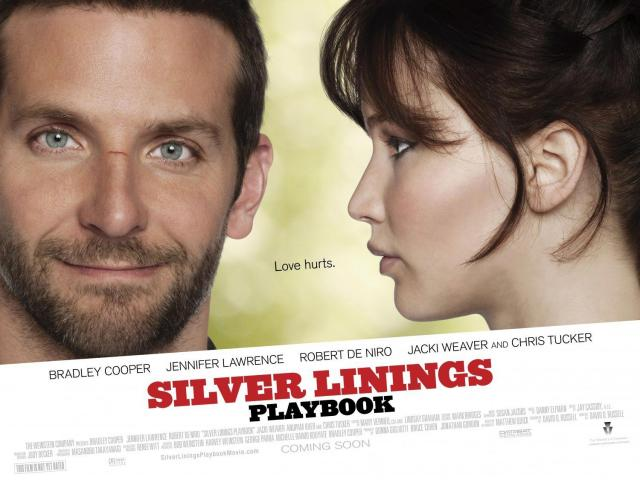
\includegraphics[width=\linewidth]{generado/q2-portador.png}
  \caption{Portador original}
\end{subfigure}\hfill
\begin{subfigure}{0.48\textwidth}
  \centering
  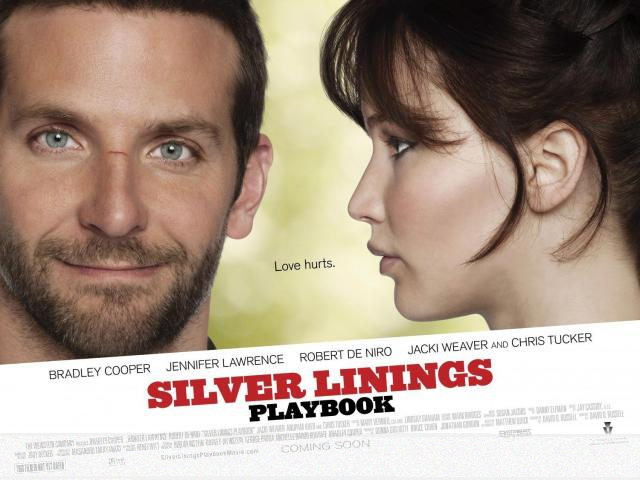
\includegraphics[width=\linewidth]{generado/q2-estego-LSB4.png}
  \caption{Con el PNG oculto usando LSB4}
\end{subfigure}
\caption{El portador y el resultado de LSB4, el método más agresivo por byte: no hay diferencia visible a simple vista}
\label{fig:q2-visual}
\end{figure}

\begin{figure}[htbp]
\centering
\begin{subfigure}{0.32\textwidth}
  \centering
  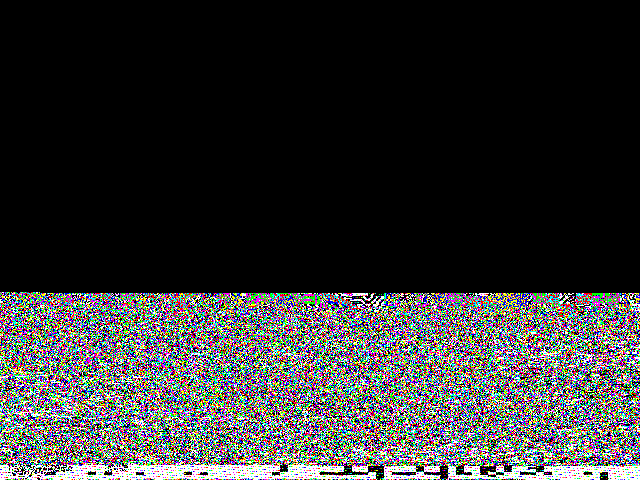
\includegraphics[width=\linewidth]{generado/q2-mapa-LSB1.png}
  \caption{LSB1}
\end{subfigure}\hfill
\begin{subfigure}{0.32\textwidth}
  \centering
  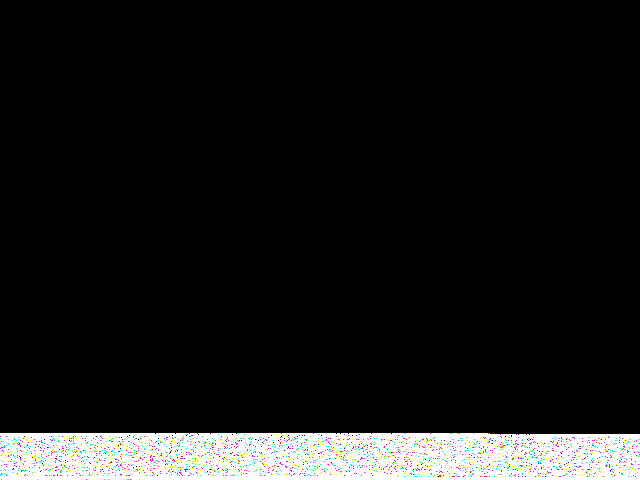
\includegraphics[width=\linewidth]{generado/q2-mapa-LSB4.png}
  \caption{LSB4}
\end{subfigure}\hfill
\begin{subfigure}{0.32\textwidth}
  \centering
  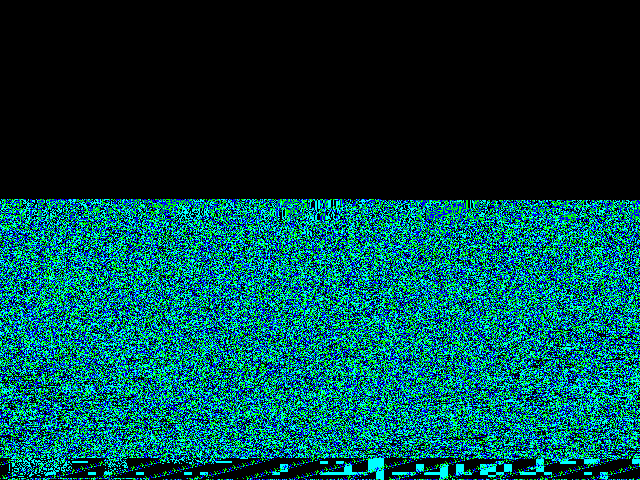
\includegraphics[width=\linewidth]{generado/q2-mapa-LSBI.png}
  \caption{LSBI}
\end{subfigure}
\caption{Mapas de cambios respecto del portador con el PNG oculto. Cada canal se enciende (rojo, verde o azul) en los píxeles donde ese byte cambió; el resto queda en negro. Las filas se muestran de arriba hacia abajo, pero el BMP guarda la fila inferior primero, así que los cambios empiezan en la parte de abajo de la imagen}
\label{fig:q2-mapas}
\end{figure}

\subsection{Análisis}

\textbf{Capacidad.} LSB4 ofrece exactamente cuatro veces la capacidad de LSB1 (\dato{cap-LSB4} contra \dato{cap-LSB1}
bytes), porque aloja cuatro bits por byte de portador en lugar de uno. LSBI queda por debajo de LSB1 (\dato{cap-LSBI}
bytes): sus bits de mensaje solo van a los bytes verde y azul, es decir, dos tercios del bloque, y además consume
cuatro bytes de portador para las banderas de los patrones invertidos. El mismo PNG ocupa el \dato{png-LSB1-uso}\,\% de la
capacidad de LSB1, el \dato{png-LSB4-uso}\,\% de la de LSB4 y el \dato{png-LSBI-uso}\,\% de la de LSBI: el método con el
mayor margen es LSB4, y LSBI es el primero que se queda sin lugar si el archivo crece.

\textbf{Distorsión por byte.} LSB1 y LSBI modifican como mucho el último bit, de modo que cada byte cambia a lo sumo en
\dato{png-LSB1-cambiomax} nivel; LSB4 reemplaza los cuatro bits bajos y un byte puede cambiar hasta
\dato{png-LSB4-cambiomax} niveles. Por eso, aunque LSB4 toca menos bytes (\dato{png-LSB4-cambiados}, contra
\dato{png-LSB1-cambiados} de LSB1 y \dato{png-LSBI-cambiados} de LSBI), su MSE es mucho mayor
(\dato{png-LSB4-mse}, contra \dato{png-LSB1-mse} y \dato{png-LSBI-mse}) y su PSNR más bajo
(\dato{png-LSB4-psnr}\,dB, contra \dato{png-LSB1-psnr}\,dB y \dato{png-LSBI-psnr}\,dB). Aun así, con esta carga LSB4
queda en un valor de PSNR que suele considerarse imperceptible, y la figura~\ref{fig:q2-visual} lo confirma a simple vista.

\textbf{Cuántos bytes cambian y dónde.} LSB4 concentra sus cambios en los primeros \dato{png-LSB4-usados} bytes del
bloque (el último byte modificado es el de posición \dato{png-LSB4-ultimo}), una franja angosta en la parte inferior de
la figura~\ref{fig:q2-mapas}. LSB1 necesita ocho bytes por byte de mensaje y los reparte en una zona cuatro veces
mayor (hasta la posición \dato{png-LSB1-ultimo}), con los tres canales por igual. LSBI llega más lejos
(\dato{png-LSBI-ultimo}) porque salta cada tercer byte, y el mapa muestra su rasgo característico: el canal rojo no se
enciende nunca (\dato{png-LSBI-rojos} bytes rojos modificados). En cambio, LSB1 modificó \dato{png-LSB1-rojos} bytes rojos
y LSB4 \dato{png-LSB4-rojos}.

\textbf{Tasa de cambio.} Sobre los bytes que efectivamente llevan mensaje, LSB1 cambió el \dato{png-LSB1-tasa}\,\%,
algo más que la mitad que resultaría de combinar bits equiprobables con bits equiprobables; la diferencia refleja que ni el
PNG ni los bits bajos del portador lo son exactamente (la proporción de unos del portador es \dato{est-portador-B-lsb} en el
canal azul). LSB4 cambió el \dato{png-LSB4-tasa}\,\%, como corresponde a reemplazar cuatro
bits: casi ningún byte coincide por casualidad, ya que con bits equiprobables solo uno de cada dieciséis lo haría. LSBI
bajó al \dato{png-LSBI-tasa}\,\% gracias a la inversión de patrones, una mejora real pero pequeña, cuyo mecanismo se
explica en la \hyperref[sec:cuestion-vii]{Cuestión VII}.

\textbf{Huellas estadísticas.} El estadístico $\chi^2$ del portador vale, por canal, \dato{est-portador-B-chi},
\dato{est-portador-G-chi} y \dato{est-portador-R-chi}; en los tres archivos cae en los canales donde se incrustó (por
ejemplo, el canal azul baja a \dato{est-png-LSB1-B-chi} con LSB1, \dato{est-png-LSB4-B-chi} con LSB4 y
\dato{est-png-LSBI-B-chi} con LSBI), porque un mensaje casi aleatorio iguala los conteos de cada par de valores. LSBI deja
el canal rojo con \dato{est-png-LSBI-R-chi}, el mismo valor del portador. Esa asimetría entre canales es coherente con
el método, pero también es una pista para quien analice el archivo. Como LSB1 y LSB4 recorren el bloque desde el primer
byte y en orden, dejan una zona inicial con estadística de azar y el resto intacto, que es justamente lo que aprovecha el
ataque de Westfeld y Pfitzmann~\cite{westfeld2000}.

\textbf{Otras cargas.} Con el mensaje del paper cambian muy pocos bytes (\dato{paper-LSB1-cambiados} con LSB1,
\dato{paper-LSB4-cambiados} con LSB4 y \dato{paper-LSBI-cambiados} con LSBI) y los tres métodos alcanzan un PSNR muy alto
(\dato{paper-LSB1-psnr}, \dato{paper-LSB4-psnr} y \dato{paper-LSBI-psnr}\,dB): en ese régimen el PSNR mide sobre todo el
tamaño del mensaje, no la calidad del método. Con datos aleatorios, que representan un mensaje cifrado, LSBI casi
deja de ganar: cambia el \dato{azar-LSBI-tasa}\,\% de los bytes usados contra el \dato{azar-LSB1-tasa}\,\% de LSB1, y la
inversión reduce los cambios de los bytes con mensaje en un \dato{inv-azar-reduccion}\,\%, valor del mismo orden que lo
esperable para bits equiprobables (unos \dato{inv-azar-teorico} cambios, el \dato{inv-azar-teoricopct}\,\%). La
ventaja de LSBI existe cuando el mensaje tiene estructura (el PNG reduce un \dato{inv-png-reduccion}\,\%, el texto
del paper un \dato{inv-paper-reduccion}\,\%), y desaparece justamente en el caso que más importa para un
programa que también cifra. Esto se reporta a propósito junto al resultado favorable del PNG y no debe leerse como
una mejora general.

\subsection{Cuadro comparativo}

El cuadro~\ref{tab:q2-ventajas} resume las ventajas y desventajas de cada método, con las cifras medidas en este
informe.

\begin{table}[htbp]
\centering
\small
\begin{tabularx}{\textwidth}{@{}l X X@{}}
\toprule
Método & Ventajas & Desventajas \\
\midrule
LSB1 &
Implementación muy simple y sin metadatos. Distorsión mínima por byte (cambio máximo de \dato{png-LSB1-cambiomax} nivel; PSNR \dato{png-LSB1-psnr}\,dB con el PNG). Usa los tres canales, con capacidad \dato{cap-LSB1} bytes. No depende de la estadística del mensaje.
&
Capacidad cuatro veces menor que la de LSB4. Modifica los tres canales y desplaza sus estadísticas, y al recorrer el portador en orden fijo desde el byte cero es detectable con el $\chi^2$ de pares de valores. Cambia cerca de la mitad de los bytes que usa (\dato{png-LSB1-tasa}\,\%). \\
\addlinespace
LSB4 &
Mayor capacidad (\dato{cap-LSB4} bytes): el PNG usa solo el \dato{png-LSB4-uso}\,\% y sus cambios se concentran en los primeros \dato{png-LSB4-usados} bytes, el \dato{png-LSB4-pctportador}\,\% del portador. Implementación igual de simple que la de LSB1.
&
Cambia casi todos los bytes que usa (\dato{png-LSB4-tasa}\,\%) y hasta \dato{png-LSB4-cambiomax} niveles, con MSE \dato{png-LSB4-mse} y PSNR \dato{png-LSB4-psnr}\,dB, el peor de los tres. La franja de cambios es compacta y fácil de localizar, y cambia la estadística de los tres canales. \\
\addlinespace
LSBI &
Menor tasa de cambio (\dato{png-LSBI-tasa}\,\%) y menor MSE (\dato{png-LSBI-mse}) que LSB1 con archivos estructurados. Deja el canal rojo intacto (\dato{png-LSBI-rojos} bytes modificados). Los cambios quedan repartidos en una zona más extensa del portador, con menor densidad local.
&
Capacidad menor (\dato{cap-LSBI} bytes) y cuatro bytes de banderas. Algoritmo más complejo (conteo por patrón y dos pasadas). La ganancia depende del mensaje: con datos aleatorios o cifrados es casi nula (\dato{inv-azar-reduccion}\,\%). El canal rojo intacto revela una asimetría entre canales. \\
\bottomrule
\end{tabularx}
\caption{Ventajas y desventajas de LSB1, LSB4 y LSBI}
\label{tab:q2-ventajas}
\end{table}

Los tres métodos comparten las mismas limitaciones de fondo: cualquier recompresión con pérdida, cambio de tamaño
o conversión de formato destruye el mensaje, y ninguno protege el contenido por sí mismo; por eso el programa ofrece
cifrado previo. Ninguno resiste un análisis estadístico dirigido: el cifrado previo protege el contenido del mensaje, pero
no su existencia.

\subsection{Conclusión de la comparación}

LSB4 conviene cuando importa la capacidad y el portador tolera una distorsión moderada: es el método con mayor margen y
el que menos superficie del portador toca, pero es el que más cambia cada byte. LSB1 es el punto medio: capacidad
suficiente para archivos medianos, distorsión mínima por byte y ninguna complejidad extra. LSBI se justifica cuando el
mensaje tiene estructura y se quiere reducir aún más la cantidad de bytes modificados sin tocar el canal rojo, a cambio de
un tercio de capacidad y de un algoritmo más delicado; si el mensaje ya está cifrado, su ventaja práctica es marginal y
LSB1 resulta más simple con resultados casi idénticos.
